\begin{adjustwidth*}{}{-2.25in}
\textbf{{\large Exercises}}
\setlength{\columnsep}{25pt}
\begin{multicols*}{2}
\noindent Terms and Concepts \small
\begin{enumerate}[1)]
\item In your own words describe what it means for a function to be increasing.
\item What does a decreasing function ``look like''?
\item Sketch a graph of a function on $[0,2]$ that is increasing but not strictly increasing.
\item Give an example of a function describing a situation where it is ``bad'' to be increasing and ``good'' to be decreasing.
\item A function $f$ has derivative $\fp(x) = (\sin(x)+2)e^{x^2+1}$, where $\fp(x) >1 $ for all $x$. Is $f$ increasing, decreasing, or can we not tell from the given information?
\item Sketch a graph of a function $f(x)$ that is:
	\ba
	\item		Increasing, concave up on $(0,1)$,
	\item		increasing, concave down on $(1,2)$,
	\item		decreasing, concave down on $(2,3)$ and 
	\item		increasing, concave down on $(3,4)$.
	\ea
\item Is is possible for a function to be increasing and concave down on $(0,\infty)$ with a horizontal asymptote of $y=1$? If so, give a sketch of such a function.
\item Is is possible for a function to be increasing and concave up on $(0,\infty)$ with a horizontal asymptote of $y=1$? If so, give a sketch of such a function.
\end{enumerate} 

\noindent {\normalsize Problems} \small

\noindent{\bf In exercises 9--18, a function is given.
\ba
\item Find the critical numbers of $f$.
\item Determine the intervals on which $f$ is increasing and decreasing.
\item Use the First Derivative Test to determine whether each critical point is a local maximum, local minimum, or neither.
\item Use the Second Derivative Test to determine whether each critical point is a local maximum, local minimum, or if the test fails.
\ea}

\begin{enumerate}[1),resume]
\item $\ds f(x) =x^2+2x-3$
	
\item $\ds f(x) =x^3+3x^2+3$
	
\item $\ds f(x) =2 x^3+x^2-x+3$

\item $\ds f(x) =x^3-3x^2+3x-1$

\item $\ds f(x) =\frac{1}{x^2-2x+2}$

\item $\ds f(x) =\frac{x^2-4}{x^2-1}$

\item $\ds f(x) =\frac{x}{x^2-2x-8}$

\item $\ds f(x) =\frac{(x-2)^{2/3}}{x}$

\item $\ds f(x) =\sin x\cos x$ on $(-\pi,\pi)$

\item $\ds f(x) =x^5-5x$
\end{enumerate}

\noindent{\bf In exercises 19--31, a function is given.
\ba
\item Find the possible points of inflection of $f$.
\item Determine the intervals on which $f$ is concave up and concave down.
\item Determine whether each possible point of inflection is in fact a point of inflection.
\ea}

\begin{enumerate}[1),resume]
\item $\ds f(x) = x^2-2x+1$ \label{exer:03_04_ex_16}
\item $\ds f(x) = -x^2-5x+7$
\item $\ds f(x) = x^3-x+1$
\item $\ds f(x) = 2x^3-3x^2+9x+5$
\item $\ds f(x) = \frac{x^4}{4}+\frac{x^3}{3}-2 x+3$
\item $\ds f(x) = -3 x^4+8 x^3+6 x^2-24 x+2$
\item $\ds f(x) = x^4-4x^3+6x^2-4x+1$
\item $\ds f(x) = \frac{1}{x^2+1}$
\item $\ds f(x) = \frac{x}{x^2-1}$
\item $\ds f(x) = \sin x + \cos x$ on $(-\pi,\pi)$
\item $\ds f(x) = x^2e^x$
\item $\ds f(x) = x^2\ln x$
\item $\ds f(x) = e^{-x^2}$\label{exer:03_04_ex_28}
\end{enumerate}

\noindent{\bf In exercises 32--45, sketch a graph of the given function using the steps outlined in the Curve Sketching Concept.}

\begin{enumerate}[1),resume]
\item $\ds f(x) = x^3-2x^2+4x+1$
\item $\ds f(x) = -x^3+5x^2-3x+2$
\item $\ds f(x) = x^3+3x^2+3x+1$
\item $\ds f(x) = x^3-x^2-x+1$
\item $\ds f(x) = (x-2)\ln (x-2)$
\item $\ds f(x) = (x-2)^2\ln (x-2)$
\item $\ds f(x) = \frac{x^2-4}{x^2}$
\item $\ds f(x) = \frac{x^2-4x+3}{x^2-6x+8}$
\item $\ds f(x) = \frac{x^2-2x+1}{x^2-6x+8}$
\item $\ds f(x) = x\sqrt{x+1}$
\item $\ds f(x) = x^2e^x$
\item $\ds f(x) = \sin x \cos x$ on $[-\pi,\pi]$
\item $\ds f(x) = (x-3)^{2/3} + 2$
\item $\ds f(x) = \frac{(x-1)^{2/3}}{x}$
\end{enumerate}

%------------------------------------------
% END OF EXERCISES ON FIRST PAGE
%------------------------------------------
\end{multicols*}
\end{adjustwidth*}

%\clearpage
%
%\begin{adjustwidth*}{}{-2.25in}
%\setlength{\columnsep}{25pt}
%\begin{multicols*}{2}\small
%
%\begin{enumerate}[1),start=12]
%
%\item \label{exer:04_02_ex_12}A rope, attached to a weight, goes up through a pulley at the ceiling and back down to a worker. The man holds the rope at the same height as the connection point between rope and weight.
%
%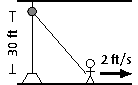
\includegraphics[scale=1.25]{figures/fig04_02_ex_12}
%
%Suppose the man stands directly next to the weight (i.e., a total rope length of 60 ft) and begins to walk away at a rate of 2ft/s. How fast is the weight rising when the man has walked:
%\begin{enumerate}
%\item	10 feet?
%\item	40 feet?
%\end{enumerate}
%How far must the man walk to raise the weight all the way to the pulley?
%
%\item Consider the situation described in Exercise \ref{exer:04_02_ex_12}. Suppose the man starts 40ft from the weight and begins to walk away at a rate of 2ft/s. 
%\begin{enumerate}
%\item	How long is the rope?
%\item	How fast is the weight rising after the man has walked 10 feet?
%\item	How fast is the weight rising after the man has walked 40 feet?
%\item	How far must the man walk to raise the weight all the way to the pulley?
%\end{enumerate}
%
%\item A company that produces landscaping materials is dumping sand into a conical pile. The sand is being poured at a rate of 5ft$^3$/sec; the physical properties of the sand, in conjunction with gravity, ensure that the cone's height is roughly 2/3 the length of the diameter of the circular base. 
%
%How fast is the cone rising when it has a height of 30 feet?
%
%\item A baseball diamond is a square with sides 90 feet long.  Suppose a baseball player is advancing from second to third base at the rate of 24 feet per second, and an umpire is standing on home plate.  Let  $\theta$ be the angle between the third baseline and the line of sight from the umpire to the runner.  How fast is $\theta$ changing when the runner is 30 feet from third base?
%	
%\item Sand is being dumped off a conveyor belt onto a pile in such a way that the pile forms in the shape of a cone whose radius is always equal to its height.  Assuming that the sand is being dumped at a rate of 10 cubic feet per minute, how fast is the height of the pile changing when there are 1000 cubic feet on the pile?
%	
%\item A swimming pool is 60 feet long and 25 feet wide. Its depth varies uniformly from 3 feet at the shallow end to 15 feet at the deep end, as shown below.
%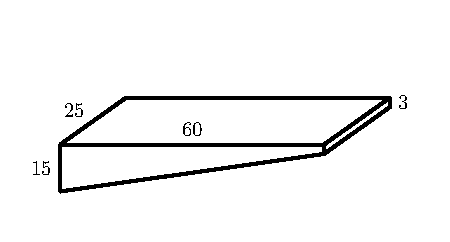
\includegraphics{figures/3_5_Ez3.eps}
%Suppose the pool has been emptied and is now being filled with water at a rate of 800 cubic feet per minute. At what rate is the depth of water (measured at the deepest point of the pool) increasing when it is 5 feet deep at that end?  Over time, describe how the depth of the water will increase:  at an increasing rate, at a decreasing rate, or at a constant rate.  Explain.
%
%\end{enumerate}
%
%%---------------------------------------------
%% END OF EXERCISES ON SECOND PAGE
%%---------------------------------------------
%\end{multicols*}
%\end{adjustwidth*}

\afterexercises